\section{Evaluation}
\label{sec:evaluation}

In this section, we present an experimental evaluation of \projecttitle based on the implementation described in  \secref{implementation}. Our evaluation answers the following questions.

\begin{itemize}
\item What overheads does \projecttitle impose for recording data provenance of multithreaded executions? ($\S$~\ref{subsec:overheads})
\item How do these overheads scale with increases in the size of input data and computation size? ($\S$~\ref{subsec:scale-overheads})
\item What are the sources for the provenance overheads? ($\S$~\ref{subsec:quantify-overheads})
\end{itemize}



\subsection{Experimental Setup}
We first describe the experimental setup used for the evaluation.

\myparagraph{Experimental platform} We used an Intel Xeon processor based
multicore architecture as our host machine for our evaluation. The
host system consists of 8 cores (16 threads) of Intel(R) Xeon(R) CPU Processor D-1540
(12M Cache, 2.00 GHz) and 32 GB of DRAM main memory. The host
machine is running Linux with kernel 4.2.0 in 64-bit mode.


\myparagraph{Applications and dataset}  We evaluated \projecttitle with applications from two multithreaded benchmark suites: Phoenix 2.0 \cite{phoenix} and PARSEC 3.0 \cite{parsec}. Table~\ref{tab:apps} lists the applications used for the evaluation along with the input data and benchmark parameters.  We report results for all 7 applications in the Phoenix benchmark and 8 out of 13 applications in the PARSEC benchmarks. %: {\em blackscholes, canneal, dedup, ferret, streamcluster, swaptions, vips,} and {\em x264}.
%The remaining five applications are not supported for the following reasons: \emph{bodytrack} and \emph{raytrace} make use of C++ exceptions, which are currently not supported by our implementation; \emph{freqmine} is an application based on OpenMP, which did not compile under our version of LLVM; \emph{fluidanimate} produces nondeterministic output and thus makes it impossible to check the correctness of the results; and finally, the native version of \emph{facesim} crashes with a runtime error when compiled with LLVM. 




\myparagraph{Metrics: Time and Work} 


\myparagraph{Measurements} All applications were compiled using GCC 4.9.2 compiler with -$o3$ optimization flag. For all performance measurements, we report the average over 10 runs with minimum and maximum values discarded.



\begin{figure}[h]
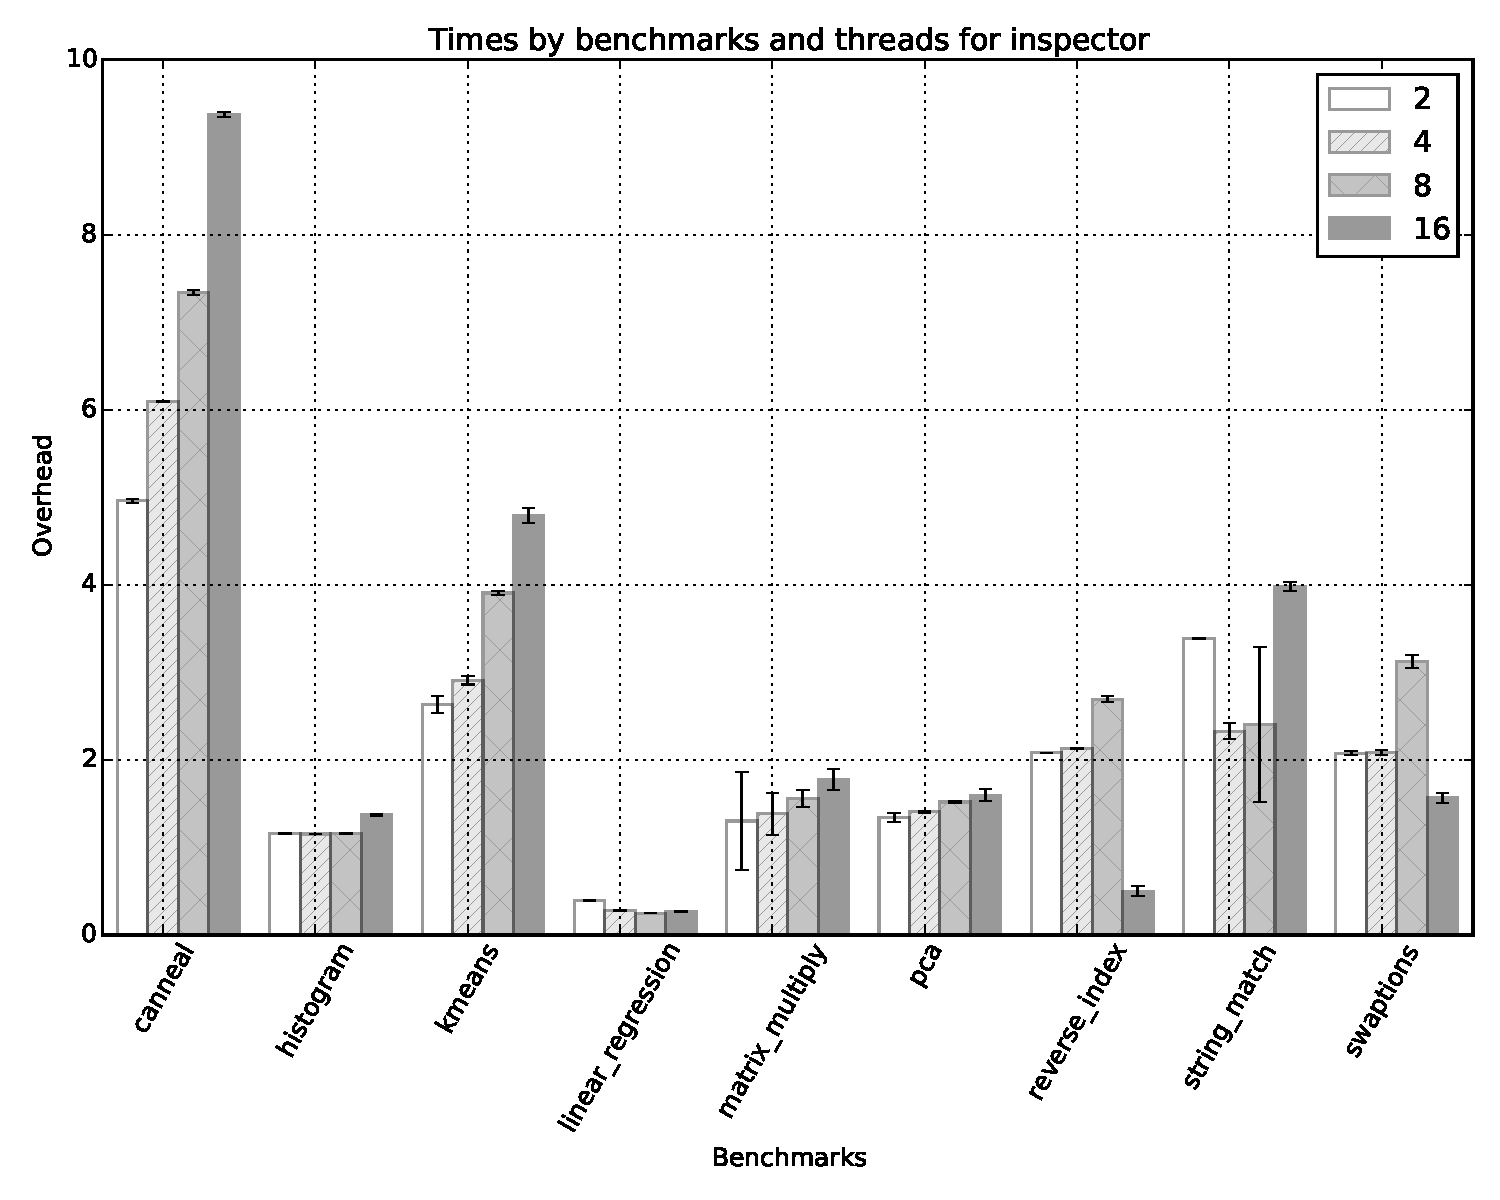
\includegraphics[width=8cm]{figure/benchmarks-inspector.pdf}
\end{figure}

\begin{figure}[h]
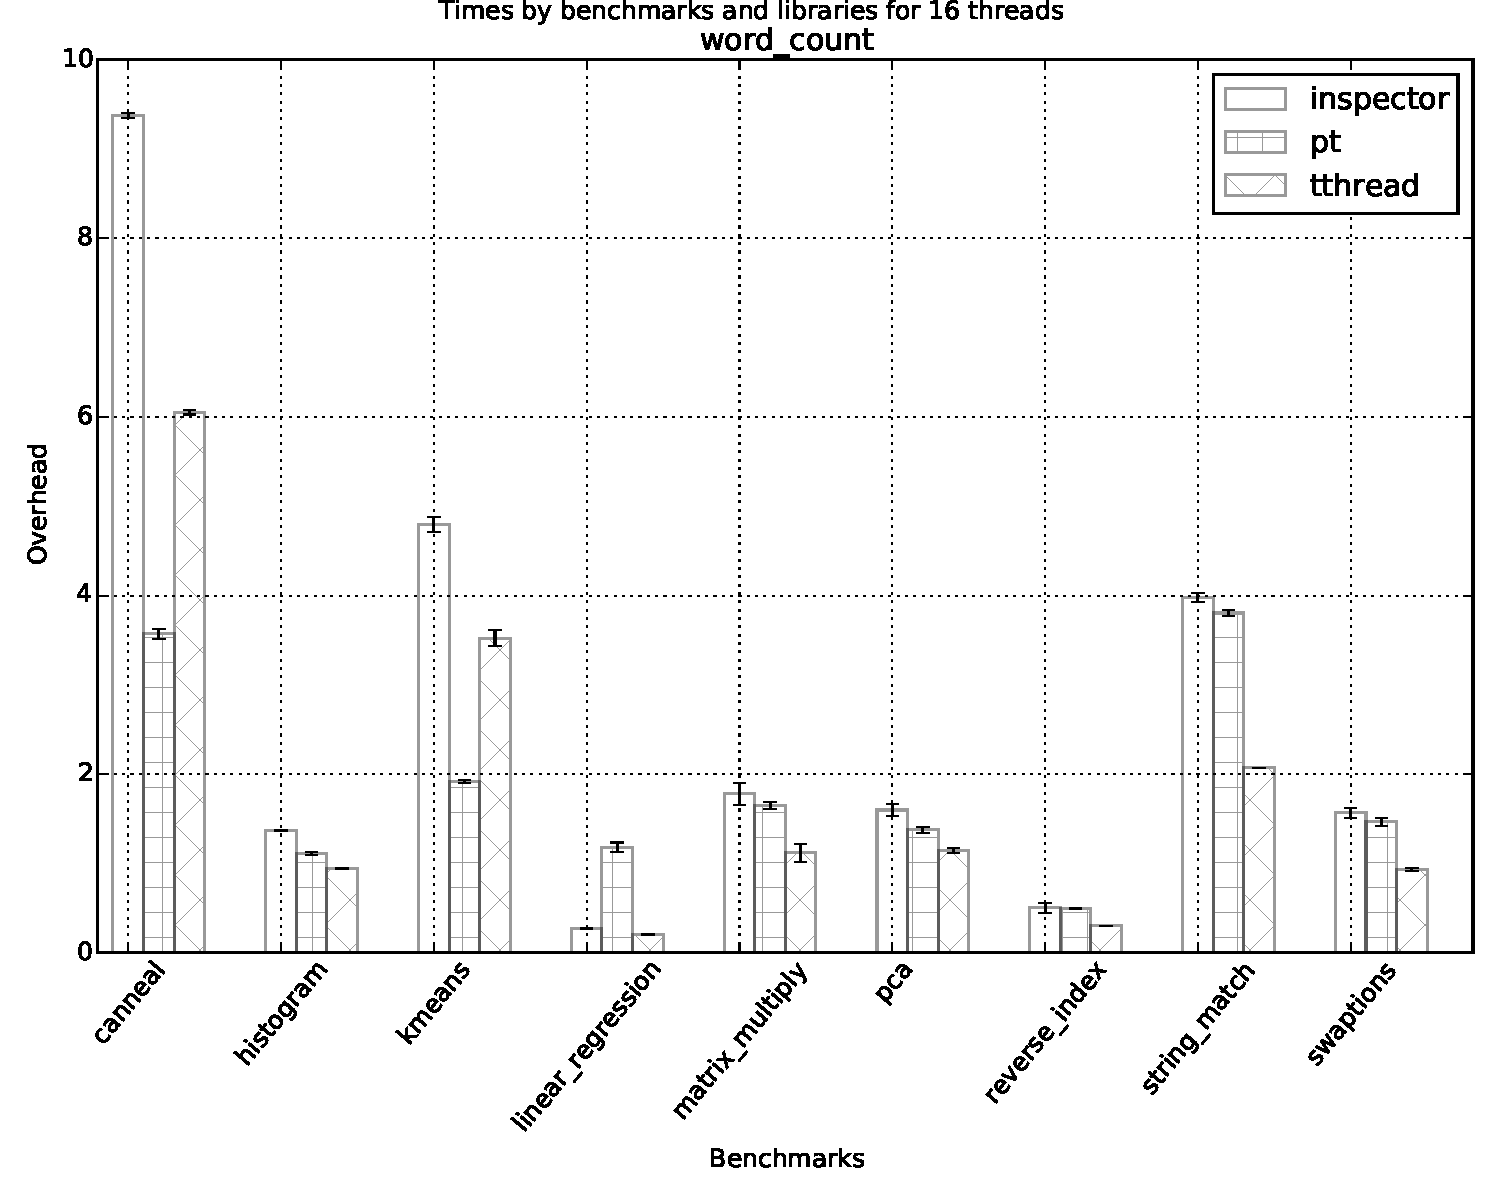
\includegraphics[width=8cm]{figure/benchmarks-16.pdf}
\end{figure}

%
%\myparagraph{Performance metrics: Work and Time}  For each run, we consider two types of measures: \emph{work} and
% {\em time}. Work refers to the total amount of
%computation performed by all threads and is measured as the total
%run-time of all threads. Time refers to the amount of (end-to-end)
%run-time to complete the parallel computation. Both metrics are important
%and complementary: time measurements reflect the end user perceived latency,
%whereas work measurements assess the overall resource (CPU) utilization.

\subsection{Provenance Overheads}

\myparagraph{Overheads}

\myparagraph{Breakdown of overheads}

\subsection{\projecttitle Scalability}

\myparagraph{Overheads w.r.t. input size}

\myparagraph{Overheads w.r.t. computation size}


\subsection{Sources of Overheads}




